\documentclass{standalone}
\usepackage{tikz}
\usetikzlibrary{patterns, positioning}

\begin{document}
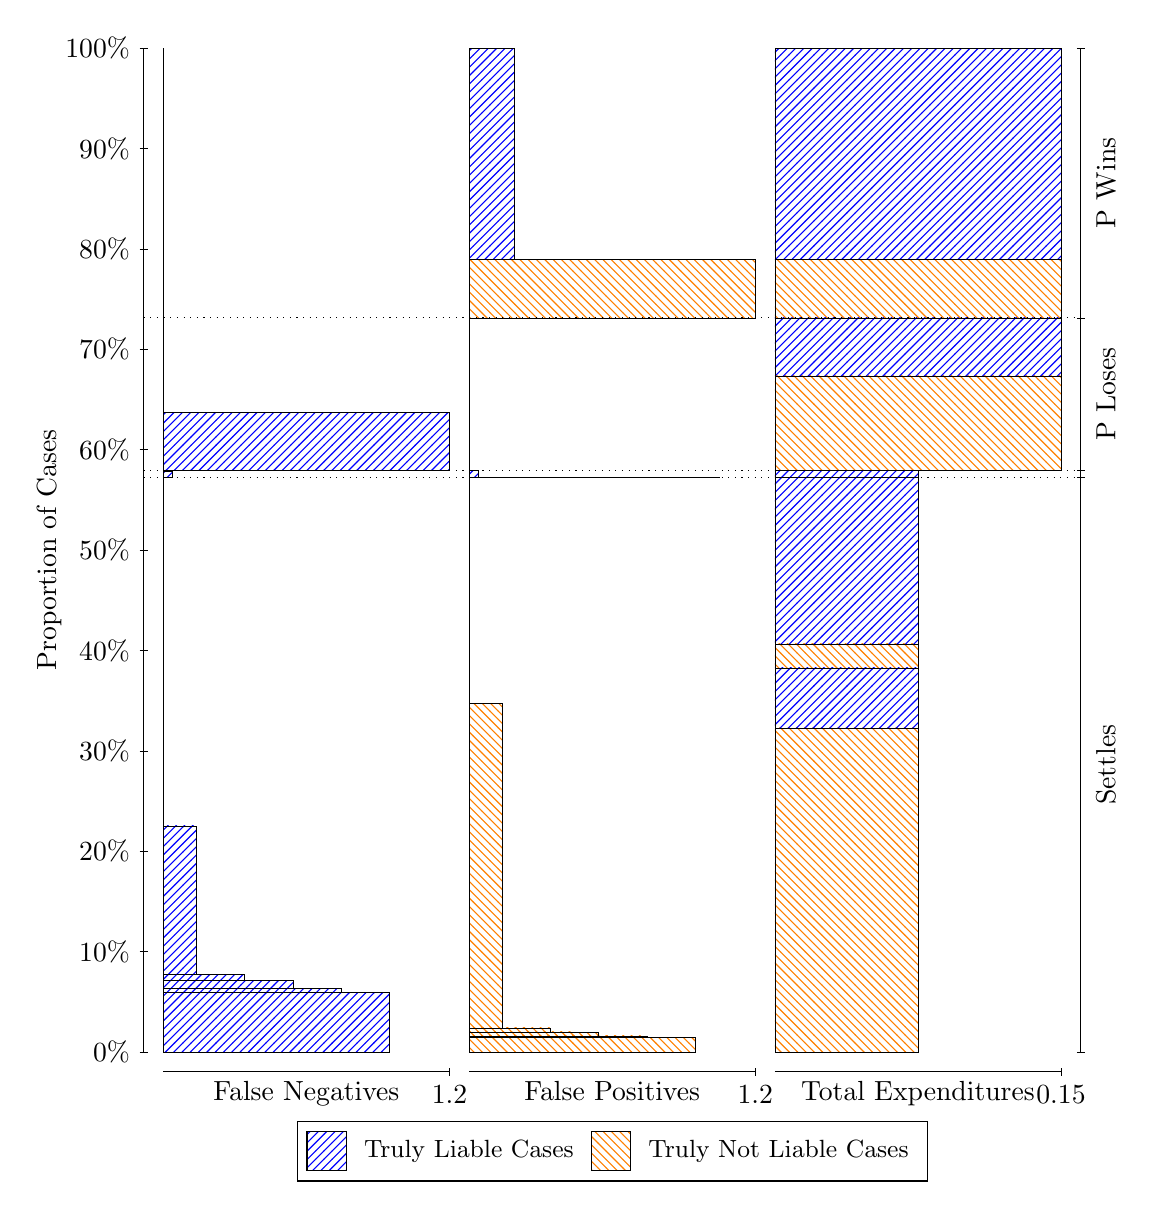
\begin{tikzpicture}
\draw[black, very thin] (1.5,1.75) -- (1.5,14.5);
\node[rotate=90, anchor=center] at (0.3, 8.125) {Proportion of Cases};
\draw[black, very thin] (1.45,1.75) -- (1.55,1.75);
\node[anchor=east] at (1.45, 1.75) {0\%};
\draw[black, very thin] (1.45,3.025) -- (1.55,3.025);
\node[anchor=east] at (1.45, 3.025) {10\%};
\draw[black, very thin] (1.45,4.3) -- (1.55,4.3);
\node[anchor=east] at (1.45, 4.3) {20\%};
\draw[black, very thin] (1.45,5.575) -- (1.55,5.575);
\node[anchor=east] at (1.45, 5.575) {30\%};
\draw[black, very thin] (1.45,6.85) -- (1.55,6.85);
\node[anchor=east] at (1.45, 6.85) {40\%};
\draw[black, very thin] (1.45,8.125) -- (1.55,8.125);
\node[anchor=east] at (1.45, 8.125) {50\%};
\draw[black, very thin] (1.45,9.4) -- (1.55,9.4);
\node[anchor=east] at (1.45, 9.4) {60\%};
\draw[black, very thin] (1.45,10.675) -- (1.55,10.675);
\node[anchor=east] at (1.45, 10.675) {70\%};
\draw[black, very thin] (1.45,11.95) -- (1.55,11.95);
\node[anchor=east] at (1.45, 11.95) {80\%};
\draw[black, very thin] (1.45,13.225) -- (1.55,13.225);
\node[anchor=east] at (1.45, 13.225) {90\%};
\draw[black, very thin] (1.45,14.5) -- (1.55,14.5);
\node[anchor=east] at (1.45, 14.5) {100\%};

\draw[black, very thin] (13.4,1.75) -- (13.4,14.5);
\draw[black, very thin] (13.35,1.75) -- (13.45,1.75);
\node[anchor=west] at (13.35, 1.75) {};
\draw[black, very thin] (13.35,9.0435) -- (13.45,9.0435);
\node[anchor=west] at (13.35, 9.0435) {};
\draw[black, very thin] (13.35,9.1366) -- (13.45,9.1366);
\node[anchor=west] at (13.35, 9.1366) {};
\draw[black, very thin] (13.35,11.073) -- (13.45,11.073);
\node[anchor=west] at (13.35, 11.073) {};
\draw[black, very thin] (13.35,14.5) -- (13.45,14.5);
\node[anchor=west] at (13.35, 14.5) {};

\draw[black, very thin, pattern color=blue, pattern=north east lines] (1.75,1.75) rectangle (4.6184,2.5094);
\draw[black, very thin, pattern color=blue, pattern=north east lines] (1.75,2.5094) rectangle (4.3125,2.5102);
\draw[black, very thin, pattern color=blue, pattern=north east lines] (1.75,2.5102) rectangle (4.0065,2.5539);
\draw[black, very thin, pattern color=blue, pattern=north east lines] (1.75,2.5539) rectangle (3.7005,2.5547);
\draw[black, very thin, pattern color=blue, pattern=north east lines] (1.75,2.5547) rectangle (3.3946,2.6561);
\draw[black, very thin, pattern color=blue, pattern=north east lines] (1.75,2.6561) rectangle (3.0886,2.6571);
\draw[black, very thin, pattern color=blue, pattern=north east lines] (1.75,2.6571) rectangle (2.7826,2.7397);
\draw[black, very thin, pattern color=blue, pattern=north east lines] (1.75,2.7397) rectangle (2.1707,4.6204);
\draw[black, very thin, pattern color=orange, pattern=north west lines] (1.75,4.6204) rectangle (1.75,9.0435);
\draw[black, very thin, pattern color=blue, pattern=north east lines] (1.75,9.0435) rectangle (1.8647,9.1281);
\draw[black, very thin, pattern color=orange, pattern=north west lines] (1.75,9.1281) rectangle (1.75,9.1366);
\draw[black, very thin, pattern color=blue, pattern=north east lines] (1.75,9.1366) rectangle (5.3833,9.8752);
\draw[black, very thin, pattern color=orange, pattern=north west lines] (1.75,9.8752) rectangle (1.75,11.073);
\draw[black, very thin, pattern color=orange, pattern=north west lines] (1.75,11.073) rectangle (1.75,11.819);
\draw[black, very thin, pattern color=blue, pattern=north east lines] (1.75,11.819) rectangle (1.75,14.5);
\draw[black, very thin, pattern color=orange, pattern=north west lines] (5.6333,1.75) rectangle (8.5018,1.9356);
\draw[black, very thin, pattern color=orange, pattern=north west lines] (5.6333,1.9356) rectangle (7.8898,1.953);
\draw[black, very thin, pattern color=orange, pattern=north west lines] (5.6333,1.953) rectangle (7.5839,1.9532);
\draw[black, very thin, pattern color=orange, pattern=north west lines] (5.6333,1.9532) rectangle (7.2779,2.0033);
\draw[black, very thin, pattern color=orange, pattern=north west lines] (5.6333,2.0033) rectangle (6.9719,2.0038);
\draw[black, very thin, pattern color=orange, pattern=north west lines] (5.6333,2.0038) rectangle (6.666,2.0561);
\draw[black, very thin, pattern color=orange, pattern=north west lines] (5.6333,2.0561) rectangle (6.36,2.0565);
\draw[black, very thin, pattern color=orange, pattern=north west lines] (5.6333,2.0565) rectangle (6.054,6.1732);
\draw[black, very thin, pattern color=blue, pattern=north east lines] (5.6333,6.1732) rectangle (5.6333,9.0435);
\draw[black, very thin, pattern color=orange, pattern=north west lines] (5.6333,9.0435) rectangle (8.8077,9.0521);
\draw[black, very thin, pattern color=blue, pattern=north east lines] (5.6333,9.0521) rectangle (5.7481,9.1366);
\draw[black, very thin, pattern color=orange, pattern=north west lines] (5.6333,9.1366) rectangle (5.6333,10.335);
\draw[black, very thin, pattern color=blue, pattern=north east lines] (5.6333,10.335) rectangle (5.6333,11.073);
\draw[black, very thin, pattern color=orange, pattern=north west lines] (5.6333,11.073) rectangle (9.2667,11.819);
\draw[black, very thin, pattern color=blue, pattern=north east lines] (5.6333,11.819) rectangle (6.207,14.5);
\draw[black, very thin, pattern color=orange, pattern=north west lines] (9.5167,1.75) rectangle (11.333,5.867);
\draw[black, very thin, pattern color=blue, pattern=north east lines] (9.5167,5.867) rectangle (11.333,6.6272);
\draw[black, very thin, pattern color=orange, pattern=north west lines] (9.5167,6.6272) rectangle (11.333,6.9333);
\draw[black, very thin, pattern color=blue, pattern=north east lines] (9.5167,6.9333) rectangle (11.333,9.0435);
\draw[black, very thin, pattern color=orange, pattern=north west lines] (9.5167,9.0435) rectangle (11.333,9.0521);
\draw[black, very thin, pattern color=blue, pattern=north east lines] (9.5167,9.0521) rectangle (11.333,9.1366);
\draw[black, very thin, pattern color=orange, pattern=north west lines] (9.5167,9.1366) rectangle (13.15,10.335);
\draw[black, very thin, pattern color=blue, pattern=north east lines] (9.5167,10.335) rectangle (13.15,11.073);
\draw[black, very thin, pattern color=orange, pattern=north west lines] (9.5167,11.073) rectangle (13.15,11.819);
\draw[black, very thin, pattern color=blue, pattern=north east lines] (9.5167,11.819) rectangle (13.15,14.5);
\draw[black, dotted] (1.5,9.0435) -- (13.4,9.0435);
\draw[black, dotted] (1.5,9.1366) -- (13.4,9.1366);
\draw[black, dotted] (1.5,11.073) -- (13.4,11.073);
\draw[black, very thin] (1.75,1.5) -- (5.3833,1.5);
\node[anchor=north] at (3.5667, 1.5) {False Negatives};
\draw[black, very thin] (5.3833,1.45) -- (5.3833,1.55);
\node[anchor=north] at (5.3833, 1.45) {1.2};

\draw[black, very thin] (5.6333,1.5) -- (9.2667,1.5);
\node[anchor=north] at (7.45, 1.5) {False Positives};
\draw[black, very thin] (9.2667,1.45) -- (9.2667,1.55);
\node[anchor=north] at (9.2667, 1.45) {1.2};

\draw[black, very thin] (9.5167,1.5) -- (13.15,1.5);
\node[anchor=north] at (11.333, 1.5) {Total Expenditures};
\draw[black, very thin] (13.15,1.45) -- (13.15,1.55);
\node[anchor=north] at (13.15, 1.45) {0.15};

\node[black, centered, rotate=90] at (13.72, 5.3968) {Settles};

\node[black, centered, rotate=90] at (13.72, 10.105) {P Loses};
\node[black, centered, rotate=90] at (13.72, 12.787) {P Wins};

\draw (7.449999999999999,1.5) node[draw=none] (baseCoordinate) {};
\begin{scope}[align=center]
        \matrix[scale=0.5, draw=black, below=0.5cm of baseCoordinate, nodes={draw}, column sep=0.1cm]{
            \node[rectangle, draw, minimum width=0.5cm, minimum height=0.5cm, pattern=north east lines, pattern color=blue] {}; &
            \node[draw=none, font=\small] (B) {Truly Liable Cases}; &
            \node[rectangle, draw, minimum width=0.5cm, minimum height=0.5cm, pattern=north west lines, pattern color=orange] {}; &
            \node[draw=none, font=\small] (B) {Truly Not Liable Cases}; \\
            };
\end{scope}

\end{tikzpicture}
\end{document}